%\subsubsection{Basicblock Window}
\label{sec:bb_window}

\textbf{BB Windows} are FIFO buffers used to store up to 16 outstanding
instructions.  Instructions in a BB Window execute in-order. In
Figure~\ref{fig:bb_arch}, eight BB Windows are shown where each BB Window can
issue up to two instructions per cycle. Each cycle, the head of each BB Window
is checked for ready instruction(s). If more than four instructions are
available, the four oldest instructions are issued. Since BB Windows are FIFO
structures, we find their lookup and update energy overhead is an order of
magnitude smaller than reservation station tables.
%justify hwy two instructions

\begin{figure}
	\centering
	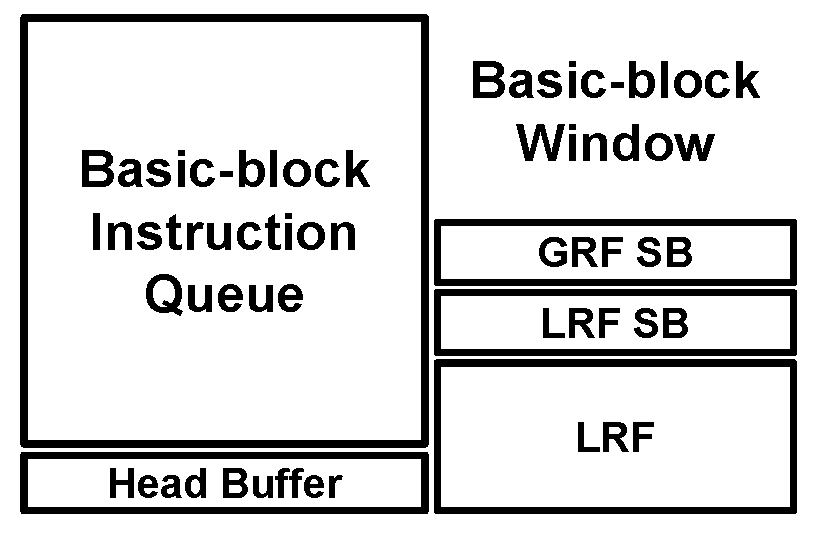
\includegraphics[width=0.6\columnwidth]{fig/bb_window.pdf} 
	\caption{Basicblock window structure}
	\label{fig:bb_window}
\end{figure}

\textbf{LRF} is a simple register file with at most 8 statically
allocated register elements. Each BB Window has its own dedicated basic-block
that is used to support storing register entries that are live only within the
basic-block lifetime. Once the basic-block completes its execution, the content
of these LRF's are invalidated. Figure~\ref{fig:bb_window} illustrates the hardware
elements supporting BB Window. GRF SB and LRF SB are the scoreboard tables used
to store the basic-block global read. A LRF SB entry is made valid once its
corresponding write operands updates the LRF. A GRF SB entry is also updated
when a global operands is about to write its valud to the GRF; the difference is a
global operand broadcasts to all GRF SB's. Since GRF SB's are small CAM arrays
with at most 7 global entries, the energy overhead of updating them is
negligible compared to an instruction window broadcast update.

Head Buffer in Figure~\ref{fig:bb_window} holds the instruction(s) pending to be
issued from the BB Window.

Figure XX shows the average number of in-flight basicblocks for SPEC2006
benchmark.

%Instructions hold offset to the instruction rather than to actual register
%address. This cuts back the register address by half (making the ISA shorter)
%    and also enable RAM lookup to the GRF table upon lookup.

%GRF scoreboard update is CAM baesd, but its lookup is RAM based. (very cheap)
%    update: CAM lookup to address ready bit
%    lookup: RAM lookup to the 1bit entry.


